\documentclass[10pt]{article}

%Math
\usepackage{amsmath}
\usepackage{amsfonts}
\usepackage{amssymb}
\usepackage{amsthm}
\usepackage{ulem}
\usepackage{stmaryrd} %f\UTF{00FC}r Blitz!

%PageStyle
\usepackage[ngerman]{babel} % deutsche Silbentrennung
\usepackage[utf8]{inputenc} 
\usepackage{fancyhdr, graphicx}
\usepackage[scaled=0.92]{helvet}
\usepackage{enumitem}
\usepackage{parskip}
\usepackage[a4paper,top=2cm]{geometry}
\setlength{\textwidth}{17cm}
\setlength{\oddsidemargin}{-0.5cm}


% Shortcommands
\newcommand{\Bold}[1]{\textbf{#1}} %Boldface
\newcommand{\Kursiv}[1]{\textit{#1}} %Italic
\newcommand{\T}[1]{\text{#1}} %Textmode
\newcommand{\Nicht}[1]{\T{\sout{$ #1 $}}} %Streicht Shit durch

%Arrows
\newcommand{\lra}{\leftrightarrow} 
\newcommand{\ra}{\rightarrow}
\newcommand{\la}{\leftarrow}
\newcommand{\lral}{\longleftrightarrow}
\newcommand{\ral}{\longrightarrow}
\newcommand{\lal}{\longleftarrow}
\newcommand{\Lra}{\Leftrightarrow}
\newcommand{\Ra}{\Rightarrow}
\newcommand{\La}{\Leftarrow}
\newcommand{\Lral}{\Longleftrightarrow}
\newcommand{\Ral}{\Longrightarrow}
\newcommand{\Lal}{\Longleftarrow}

\newcommand{\BN}{\mathfrak{B}} %Belegung
\newcommand{\RN}{\mathbb{R}} %Real Number
\newcommand{\NN}{\mathbb{N}} %Natural Number
\newcommand{\QN}{\mathbb{Q}} %Rational Number
\newcommand{\ZN}{\mathbb{Z}} %ganze Zahlen
\newcommand{\CN}{\mathbb{C}}

% Code listenings
\usepackage{color}
\usepackage{xcolor}
\usepackage{listings}
\usepackage{caption}
\DeclareCaptionFont{white}{\color{white}}
\DeclareCaptionFormat{listing}{\colorbox{gray}{\parbox{\textwidth}{#1#2#3}}}
\captionsetup[lstlisting]{format=listing,labelfont=white,textfont=white}
\lstdefinestyle{CStyle}{
 language=Java,
 basicstyle=\footnotesize\ttfamily, % Standardschrift
 numbers=left,               % Ort der Zeilennummern
 numberstyle=\tiny,          % Stil der Zeilennummern
 stepnumber=5,              % Abstand zwischen den Zeilennummern
 numbersep=5pt,              % Abstand der Nummern zum Text
 tabsize=2,                  % Groesse von Tabs
 extendedchars=true,         %
 breaklines=true,            % Zeilen werden Umgebrochen
 frame=b,         
 %commentstyle=\itshape\color{LightLime}, Was isch das? O_o
 %keywordstyle=\bfseries\color{DarkPurple}, und das O_o
 basicstyle=\footnotesize\ttfamily,
 stringstyle=\color[RGB]{42,0,255}\ttfamily, % Farbe der String
 keywordstyle=\color[RGB]{127,0,85}\ttfamily, % Farbe der Keywords
 commentstyle=\color[RGB]{63,127,95}\ttfamily, % Farbe des Kommentars
 showspaces=false,           % Leerzeichen anzeigen ?
 showtabs=false,             % Tabs anzeigen ?
 xleftmargin=17pt,
 framexleftmargin=17pt,
 framexrightmargin=5pt,
 framexbottommargin=4pt,
 showstringspaces=false      % Leerzeichen in Strings anzeigen ?        
}

%Config
\renewcommand{\headrulewidth}{0pt}
\setlength{\headheight}{15.2pt}

%Metadata
\fancyfoot[C]{If you use this documentation for a exam, you should offer a beer to the authors!}
\title{
	\vspace{5cm}
	Computergrafik
}
\author{Jan Fässler}
\date{5. Semester (HS 2013)}


% hier beginnt das Dokument
\begin{document}

% Titelbild
\maketitle
\thispagestyle{fancy}

\newpage

% Inhaltsverzeichnis
\pagenumbering{Roman}
\tableofcontents	  	


\newpage
\setcounter{page}{1}
\pagenumbering{arabic}

% Inhalt Start

\section{Mathematische Grundlagen}
\subsection{Euklidischer Raum}
\begin{itemize}
	\item OpenGL benutzt das rechtshändige Koordinatensystem. Direct3D oder der Raytracer POVRay benutzen das links-händige System.
	\item Nehmen Sie die rechte Hand, streckt den Daumen nach rechts, den Zeigefinger nach oben und den Mittelfinger nach vorne.
	\item Die Finger zeigen dabei in die positiven Richtungen der x-, y- und z-Achse.
	\item Die Drehwinkel werden im Gegenuhrzeigersinn 	gemessen.
\end{itemize}
\begin{center}
	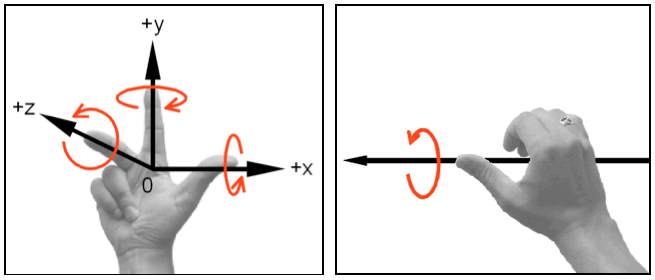
\includegraphics[scale=0.4]{euklidischer_raum.png}
\end{center}

\subsection{Vektoren}
\begin{itemize}
	\item Vektoren haben eine Richtung und eine Länge aber KEIN Ort.
	\item Punkte im Raum können durch Ortsvektoren beschrieben werden.
	\item Sie werden als n-Tupel, als geordnete Liste von reellen Zahlen beschrieben
	\item Punkte sind Orte, Vektoren sind Richtungen
\end{itemize}
\begin{center}
	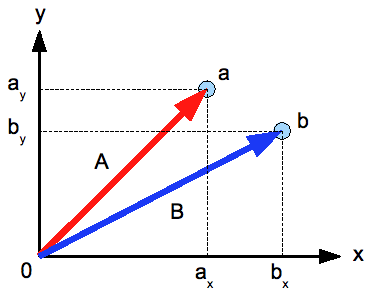
\includegraphics[scale=0.4]{vektoren.png}
\end{center}
\subsubsection{Addition}
\begin{equation}
	C=A+B=
	\begin{bmatrix}
	a_0+b_0 \\
	a_1+b_1 \\
	\dots \\
	 a_{n-1} + b_{n-1}
	\end{bmatrix}	
	\in \RN^n	
\end{equation}
\subsubsection{skalare Multiplikation}
\begin{equation}
	s*A=
	\begin{bmatrix}
	s*a_0 \\
	s*a_1 \\
	\dots \\
	s*a_{n-1}
	\end{bmatrix}
	\in \RN^n
\end{equation}
\subsubsection{Betrag}
\begin{equation}
	\text{Länge}=|A|=\sqrt{A * A} = \sqrt{a_0^2+a_1^2+\dots+a_{n-1}^2}
\end{equation}
\subsubsection{Einheitsvektor}
Ein Vektor mit der Länge 1 wird Einheitsvektor bezeichnet
\begin{equation}
	E =\frac{1}{|A|} * A = \frac{1}{\sqrt{a_0^2+a_1^2+\dots+a_{n-1}^2}} * 
	\begin{bmatrix}
	a_0 \\ a_1 \\ \dots \\ a_{n-1}
	\end{bmatrix}
\end{equation}
\subsubsection{Skalarprodukt}
\begin{equation}
	A \bullet B = |A| * |B| + cos(\alpha)
\end{equation}
\begin{equation}
	cos(\alpha)=\frac{A \bullet B}{|A| * |B| }
\end{equation}
\begin{equation}
	cos(\alpha)=\frac{p}{|A|}
\end{equation}
\begin{equation}
	\text{Projektion} = p=cos(\alpha) * |A| = \frac{A \bullet B}{|B|}
\end{equation}
\subsubsection{Vektorprodukt}
Der resultierende Vektor N steht senkrecht auf den Vektoren A und B
\begin{equation}
	N= A \times B =
	\begin{bmatrix}
	a_1 * b_2 - a_2 * b_1 \\
	a_2 * b_0 - a_0 * b_2 \\
	a_0 * b_1 - a_1 * b_0
	\end{bmatrix}
	\in \RN^n
\end{equation}

\subsection{Matrizen}
Eine Matrix ist ein rechteckiges Schema von reellen Zahlen mit nx Zeilen und ny Spalten
\begin{equation}
A_{nx \times ny} = 
\begin{bmatrix}
	a_{0,0} & a_{0,1} & \dots & a_{0,ny-1} \\
	a_{1,0} & a_{1,1} & \dots & a_{1,ny-1} \\
	\vdots & \vdots & \ddots & \vdots \\
	a_{nx-1,0} & a_{nx-1,1} & \dots & a_{nx-1,ny-1} \\
\end{bmatrix}
\end{equation}
\subsubsection{Einheitsmatrix}
Wird ein Vektor damit transformiert resultiert daraus derselbe Vektor
\begin{equation}
I=
\begin{bmatrix}
 1 & 0 & \dots & 0 \\
 0 & 1 & \dots & 0 \\
 \vdots & \vdots & \ddots & \vdots \\
 0 & 0 & \dots & 1
\end{bmatrix}
\end{equation}
\subsubsection{Transponierte Matrix}
Bei der transponierten Matrix sind die Spalten und Zeilen vertauscht
\begin{equation}
A_{nx \times ny}^T = 
\begin{bmatrix}
	a_{0,0} & a_{1,0} & \dots & a_{nx-1,0} \\
	a_{0,1} & a_{1,1} & \dots & a_{nx-1,1} \\
	\vdots & \vdots & \ddots & \vdots \\
	a_{0,ny-1} & a_{1,ny-1} & \dots & a_{nx-1,ny-1} \\
\end{bmatrix}
\end{equation}
\subsubsection{Multiplikation}
\begin{align}
C_{m \times p} &= A_{m \times n} * B_{n \times p} \\ 
& =
\begin{bmatrix}
a_{0,0} & \dots & a_{a,n-1} \\
\vdots & \ddots & \vdots \\
a_{m-1,0} & \dots & a_{m-1, n-1}
\end{bmatrix} *
\begin{bmatrix}
a_{0,0} & \dots & a_{a,p-1} \\
\vdots & \ddots & \vdots \\
a_{n-1,0} & \dots & a_{n-1, p-1}
\end{bmatrix} \\
& =
\begin{bmatrix}
\sum_{i=0}^{n-1} a_{0,i} * b_{i,0} & \dots & \sum_{i=0}^{n-1} a_{0,i} * b_{i,p-1} \\
\vdots & \ddots & \vdots \\
\sum_{i=0}^{m-1} a_{0,i} * b_{i,0} & \dots & \sum_{i=0}^{n-1} a_{m-1,i} * b_{i,p-1}
\end{bmatrix}
\end{align}

\subsection{Homogene Koordinaten}
Man kann Transformationen einfacher handhaben und miteinander kombinieren, wenn sie sich alle einheitlich, durch eine Multiplikation beschreiben liessen. Dies lässt sich durch sogenannte homogene Koordinaten erreichen. In der homogenen Darstellung werden die Koordinaten des Punktes P um eine weitere Komponente w ergänzt. \\
\begin{equation}
P= \begin{bmatrix}
x \\ y \\ w
\end{bmatrix}
\end{equation}
Mit homogenen Koordinaten gibt es unendlich viele Repräsentationen eines Punktes. Die Normalisierung wird mit der Division durch w erreicht. Um diesen Schritt zu umgehen, benutzt man deshalb die Standarddarstellung mit $w=1.0$. Ist die Komponente $w=0$, so liegt der repräsentierte Punkt im Unendlichen (Division durch 0!). Seine Koordinaten legen dann lediglich die Richtung fest, in der der Punkt im Unendlichen liegt.

\subsection{2D-Transformationen}
\subsubsection{Translation}
\begin{equation}
\begin{bmatrix} x' \\ y' \\ 1\end{bmatrix}
= \begin{bmatrix}
1 & 0 & t_x \\
0 & 1 & t_y \\
0 & 0 & 1
\end{bmatrix} * \begin{bmatrix} x \\ y \\ 1\end{bmatrix}
\end{equation}
\subsubsection{Skalierung}
\begin{equation}
\begin{bmatrix} x' \\ y' \\ 1\end{bmatrix}
= \begin{bmatrix}
s_x & 0 & 0\\
0 & s_y & 0 \\
0 & 0 & 1
\end{bmatrix} * \begin{bmatrix} x \\ y \\ 1\end{bmatrix}
\end{equation}
\subsubsection{Scherung}
\begin{equation}
\begin{bmatrix} x' \\ y' \\ 1\end{bmatrix}
= \begin{bmatrix}
1 & h_{xy} & 0\\
h_{xy} & 1 & 0\\
0 & 0 & 1
\end{bmatrix} * \begin{bmatrix} x \\ y \\ 1\end{bmatrix}
\end{equation}
\subsubsection{Rotation}
\begin{equation}
\begin{bmatrix} x' \\ y' \\ 1\end{bmatrix}
= \begin{bmatrix}
cos(\varphi) & -sin(\varphi) & 0 \\
sin(\varphi) & cos(\varphi) & 0\\
0 & 0 & 1
\end{bmatrix} * \begin{bmatrix} x \\ y  \\ z\\ 1\end{bmatrix}
\end{equation}

\subsection{3D-Transformationen}
\subsubsection{Translation}
\begin{equation}
\begin{bmatrix} x' \\ y' \\ z'\\ 1\end{bmatrix}
= \begin{bmatrix}
1 & 0 & 0 & t_x \\
0 & 1 & 0 & t_y \\
0 & 0 & 1 & t_z \\
0 & 0 & 0 & 1
\end{bmatrix} * \begin{bmatrix} x \\ y  \\ z\\ 1\end{bmatrix}\end{equation}
\subsubsection{Skalierung}
\begin{equation}
\begin{bmatrix} x' \\ y' \\ z'\\ 1\end{bmatrix}
= \begin{bmatrix}
s_x & 0 & 0 & 0\\
0 & s_y & 0 & 0 \\
0 & 0 & s_z & 0 \\
0 & 0 & 0 & 1
\end{bmatrix} * \begin{bmatrix} x \\ y  \\ z\\ 1\end{bmatrix}\end{equation}
\subsubsection{Scherung}
\begin{equation}
\begin{bmatrix} x' \\ y' \\ z'\\ 1\end{bmatrix}
= \begin{bmatrix}
1 & h_{xy} & h_{xz} & 0\\
h_{xy} & 1 & h_{yz} & 0\\
h_{zx} & h_{zy} & 1 & 0\\
0 & 0 & 0 & 1
\end{bmatrix} * \begin{bmatrix} x \\ y  \\ z\\ 1\end{bmatrix}\end{equation}
\subsubsection{Rotation}
Rotation um die x-Achse:
\begin{equation}
\begin{bmatrix} x' \\ y' \\ z'\\ 1\end{bmatrix}
= \begin{bmatrix}
1 & 0 & 0 & 0\\	
0 & cos(\varphi) & -sin(\varphi) & 0 \\
0 & sin(\varphi) & cos(\varphi)  & 0\\
0 & 0 & 0 & 1
\end{bmatrix} * \begin{bmatrix} x \\ y  \\ z\\ 1\end{bmatrix}\end{equation}
Rotation um die y-Achse:
\begin{equation}
\begin{bmatrix} x' \\ y' \\ z'\\ 1\end{bmatrix}
= \begin{bmatrix}
cos(\varphi) & 0  & sin(\varphi) & 0 \\
0 & 1 & 0 & 0 \\
-sin(\varphi) & 0 & cos(\varphi)  & 0\\
0 & 0 & 0 & 1
\end{bmatrix} * \begin{bmatrix} x \\ y  \\ z\\ 1\end{bmatrix}\end{equation}
Rotation um die z-Achse:
\begin{equation}
\begin{bmatrix} x' \\ y' \\ z'\\ 1\end{bmatrix}
= \begin{bmatrix}
cos(\varphi) & -sin(\varphi) & 0 & 0 \\
sin(\varphi) & cos(\varphi) & 0 & 0\\
0 & 0 & 1 & 1\\
0 & 0 & 0 & 1
\end{bmatrix} * \begin{bmatrix} x \\ y  \\ z\\ 1\end{bmatrix}\end{equation}
\subsubsection{Rotation um eine beliebige Achse}
\begin{enumerate}
	\item Drehen um $\alpha$ um die x-Achse
	\item Drehen um $-\beta$ um die y-Achse
	\item Drehen um $\varphi$ um die z-Achse
	\item Raum zurückdrehen: $\beta$ um y-Achse, $-\alpha$ um x Achse
\end{enumerate}
\begin{center}
	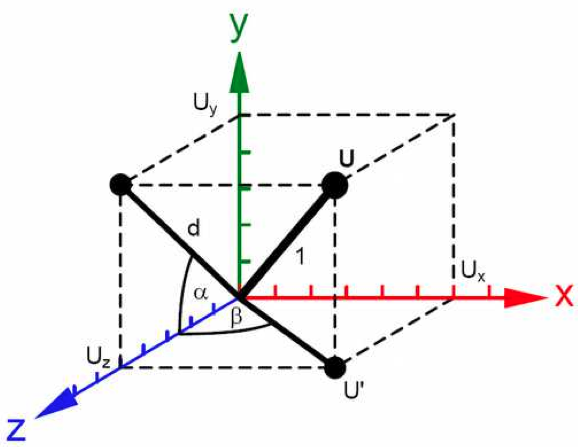
\includegraphics[scale=0.3]{rotation.png}
\end{center}

\newpage
\section{Rasteralgorithmen}
\subsection{Inkrementeller Algorithmus}
\lstinputlisting[style=CStyle,caption=Inkrementeller Algorithmus]{line_increment.c}
\subsection{Bresenham Algorithmus}
\begin{center}
	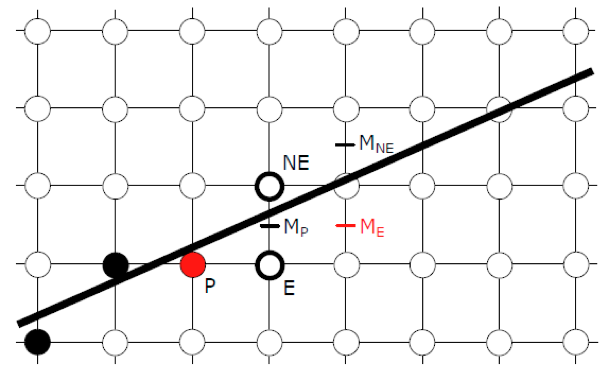
\includegraphics[scale=0.4]{bersenhan.png}
\end{center}
\lstinputlisting[style=CStyle,caption=Bresenham Algorithmus]{bersenhan.c}

\newpage
\section{Perspektive: 3D auf 2D}
\subsection{Kategorien der Projektionen}
Es gibt zwei Arten von Projektionen: perspektivische und parallele. Bei Parallelprojektionen ist der Blickpunkt unendlich weit entfernt, wodurch sich parallele Projektionsstrahlen ergeben. Im Gegensatz dazu führen die Projektionsstrahlen bei Zentralprojektionen ins Zentrum, in den Blickpunkt.
\begin{center}
	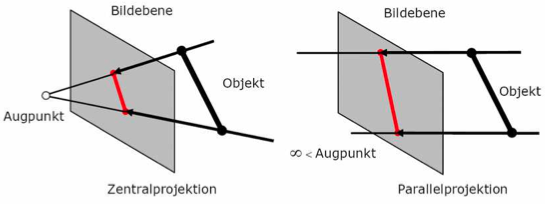
\includegraphics[scale=0.4]{projektionen.png}
\end{center}
\subsection{Parallelprojektion}
Bei Parallelprojektionen sind die Projektionsstrahlen parallel zueinander. Sie können gegen die Projektionsebene schief oder senkrecht (orthogonal) stehen. Parallelprojektionen werden vor allem in technischen Zeichnungen verwendet, um die Tiefeninformationen ablesbar zu halten. Im Gegensatz zur Perspektive sind weiter entfernte Objekte nicht kleiner als nahe Objekte. 
\begin{center}
	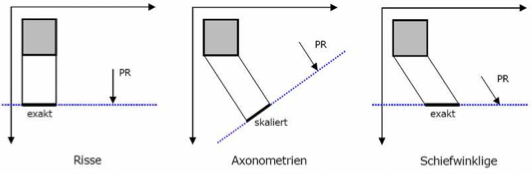
\includegraphics[scale=0.4]{parallelprojektion.png}
\end{center}
\subsection{Zentralprojektion}
Durch die Zusammenführung der Projektionsstrahlen im Projektionszentrum entsteht eine optische Tiefenwirkung. Das Sichtvolumen (Englisch für View Frustum) entspricht bei der perspektivischen Projektion einem Pyramidenstumpf. Es wird wie das orthogonale Sichtvolumen durch die Parameter t=top, l=left, r=right, b=bottom, n=near und f=far definiert:
\begin{center}
	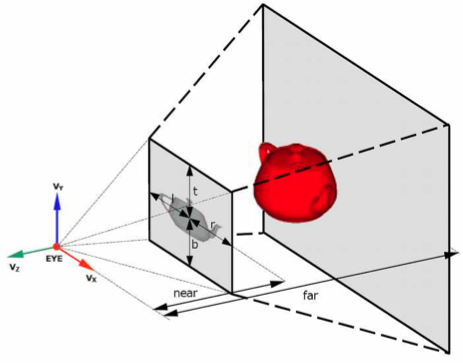
\includegraphics[scale=0.4]{zentralprojektion.png}
\end{center}
\subsection{Projektionstransformation}
Wir können View-Koordinaten nicht auf die Near-Clipping Plane projizieren. Ein zusätzlicher Schritt, die perspektivische Normalisierung ist notwendig. Die perspektivische Transformation kann in vier Schritte zerlegen werden:
\begin{enumerate}
	\item Scherung H in eine orthogonale Sichtpyramide
	\item Skalierung S in ein kanonisches Sichtvolumen
	\item Projektive Transformation N in einen Sichtwürfel 
	\item Perspektivische Division
\end{enumerate}
\subsubsection{Schritt 1: Scherung H in eine orthogonale Sichtpyramide}
Ist die Blickrichtung (Mittellinie der Pyramide) nicht parallel zur negativen z-Achse und somit nicht rechtwinklig zur Projektionsfläche, so muss sie zuerst mit einer Scherung H mit der z-Achse in Übereinstimmung gebracht werden.
\begin{center}
	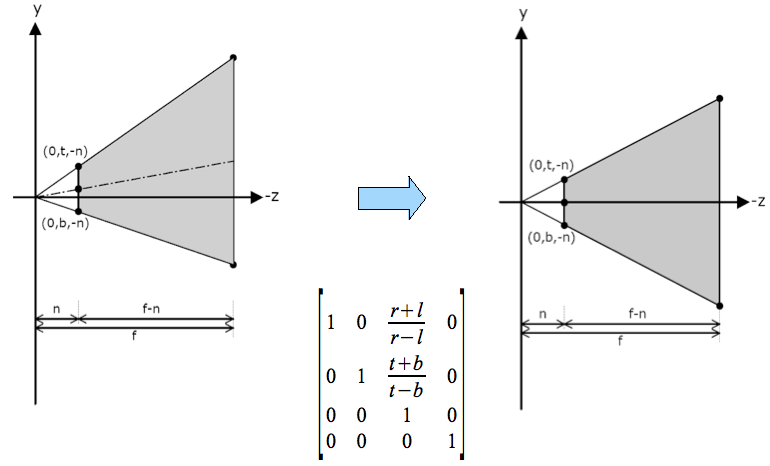
\includegraphics[scale=0.2]{projektionstransformation1.png}
\end{center}
\subsubsection{Skalierung S in ein kanonisches Sichtvolumen}
Stimmt die Blickrichtung mit der negativen z-Achse überein, so wird zur Vereinfachung der perspektivischen Normalisierung im nächsten Schritt mit einer Skalierung S das Sichtvolumen in eine Sichtpyramide transformiert. Die Skalierung betrifft ebenfalls nur die x- und y-Koordinaten.
\begin{center}
	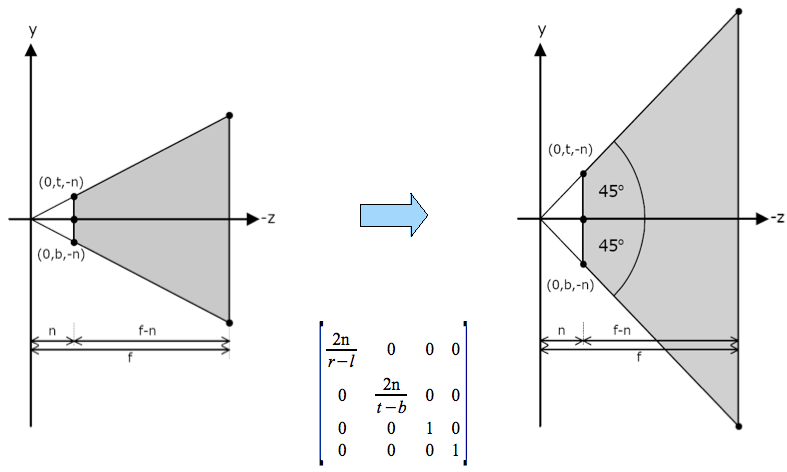
\includegraphics[scale=0.2]{projektionstransformation2.png}
\end{center}
\subsubsection{Projektive Transformation N in einen Sichtwürfel }
\begin{center}
	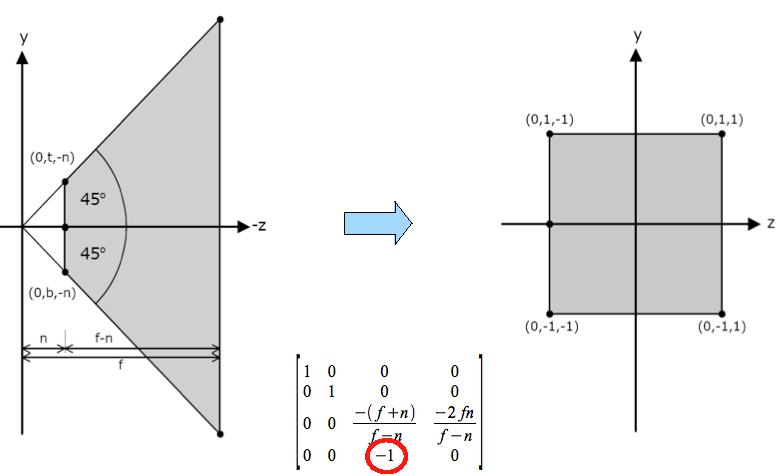
\includegraphics[scale=0.2]{projektionstransformation3.png}
\end{center}
\subsubsection{Perspektivische Division}
Die perspektivische Projektion transformiert die View-Koordinaten in homogene sogenannte Clip-Koordinaten ($C_X$, $C_Y$, $C_Z$, $C_W$). Mit diesen Koordinaten wird in einem nächsten Zwischenschritt das 3D-Clipping durchgeführt. Polygone, die aus der Projektionsebene hinausragen, werden abgeschnitten.
\begin{center}
	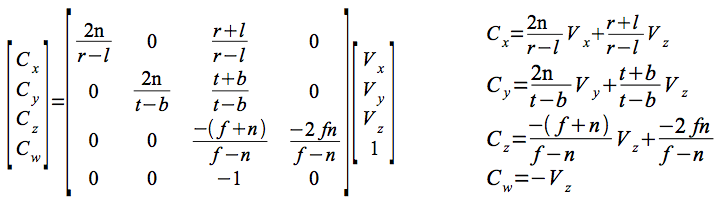
\includegraphics[scale=0.3]{projektionstransformation4_1.png}
\end{center}
Um die gewünschten normalisierten Device-Koordinaten (NDC) ($D_X$, $D_Y$, $D_Z$) zu erhalten, muss nach dem Clipping die Division durch $C_W$ durchgeführt werden. Dieser Schritt wird auch perspektivische Division genannt:
\begin{center}
	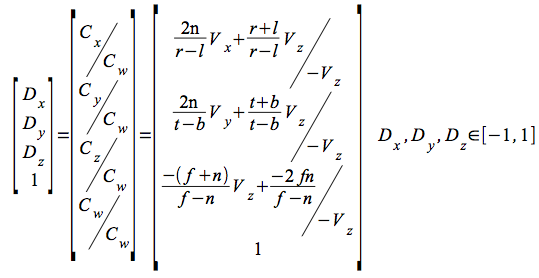
\includegraphics[scale=0.3]{projektionstransformation4_2.png}
\end{center}
\subsection{Viewport-Transformation}
Wir sind mit der Projektionstransformation noch nicht ganz am Ende angelangt. Es fehlt noch die Umrechnung von den normalisierten Device-Koordinaten ($D_X$, $D_Y$, $D_Z$) der virtuellen Projektionsebene zu den Fensterkoordinaten ($S_X$, $S_Y$) und dem Tiefenbufferwert $S_Z$ zwischen $n$ und $f$. Für ein Fenster mit den Fensterkoordinaten von $[x, y]$ unten-links bis $[ww, wh]$ oben-rechts und einem Tiefenbuffer mit Werten zwischen $n$ und $f$ (bei OpenGL normalerweise 0-1) ergäbe sich eine Viewport-Matrix wie folgt:
\begin{equation}
\begin{bmatrix}
S_x \in [x, ww] \\
S_y \in [y, wh] \\
S_z \in [n, f] \\
1
\end{bmatrix} = \begin{bmatrix}
\frac{ww}{2} & 0 & 0 & \frac{x + ww}{2} \\
0 & \frac{wh}{2} & 0 & \frac{y + wh}{2} \\
0 & 0 & \frac{f - n}{2} & \frac{f + n}{2} \\
0 & 0 & 0 & 1
\end{bmatrix}
\end{equation}
\begin{center}
	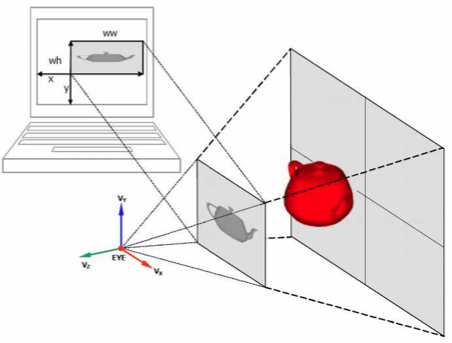
\includegraphics[scale=0.5]{viewport_transformation.png}
\end{center}

\newpage
\section{OpenGL}
\subsection{Was ist OpenGL?}
OpenGL ist ein Software-Interface zur Grafik-Hardware. Das Ziel ist die Echtzeitdarstellung (\textbf{Realtime Rendering}) von \textbf{2D- und 3D-Objekten}. Die Objekte werden durch Raumpunkte (\textbf{Vertizes}) definiert und können durch eine beliebige Transformation auf ein Ausgaberechteck (\textbf{Viewport}) projiziert werden. Die Farbe von jedem Pixel im Ausgabebild kann durch Berechnung und/oder durch Belegung mit Rasterbildern (\textbf{Texture Mapping}) bestimmt werden. \\
OpenGL bietet keine Funktionalität für die Anbindung an ein GUI oder andere betriebssystemabhängige Dienste. Diese werden von den jeweiligen Betriebssystemen bereitgestellt. OpenGL bietet nur primitive geometrische Objekte (Punkte, Linien und Dreiecke) an. \\
OpenGL ist eine Zustandsmaschine (\textbf{State Machine}). Zu jedem Zeitpunkt des Rendering-Prozesses herrscht ein gültiger Zustand. Wird ein Zustand durch ein Ereignis verändert, gilt dieser für alle nachfolgenden Objekte so lange, bis der Zustand wieder verändert wird. Das Setzen der aktuellen Farbe bestimmt z. B. den Zustand der Farbe. Dieser gilt fortan für alle folgenden Objekte, bis der Farbzustand wieder verändert wird. Jede Zustandsvariable hat einen Defaultwert. Der aktuelle Wert eines Zustandes kann mit einer \textbf{glGet*()} Funktion abgefragt werden. Bestimmte Zustände können aktiviert oder deaktiviert werden mit \textbf{glEnable} und \textbf{glDisable}. \\
Das OpenGL API funktioniert nach dem Client/Server Modell, wobei der Client die Applikation und die OpenGL- Implementation der Server ist.
\subsection{Rendering Pipeline}
\begin{center}
	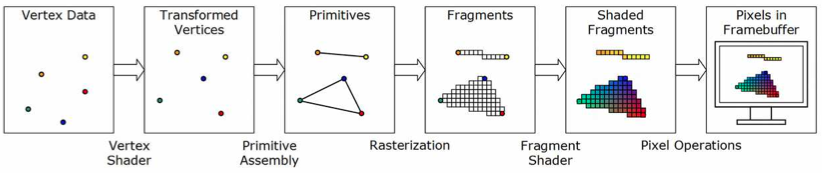
\includegraphics[scale=0.5]{rendering_pipline.png}
	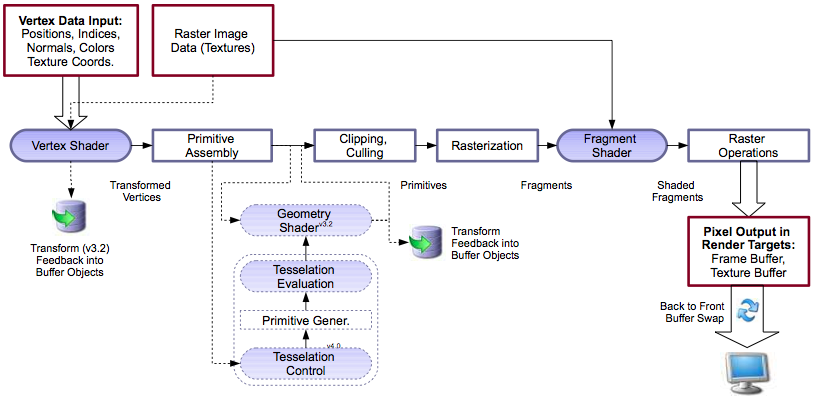
\includegraphics[scale=0.5]{rendering_pipline2.png}
\end{center}
\subsection{Shaders}
Bei der Initialisierung in \textbf{onInit} werden der Quellcode des Vertex Shaders und des Fragment Shaders mit \textbf{loadShader} geladen und mit \textbf{buildShader} und \textbf{buildProgram} kompiliert und zu einem Programm gelinkt.
\lstinputlisting[style=CStyle,caption=Minimaler Vertex Shader]{min.vert}
\lstinputlisting[style=CStyle,caption=Minimaler Fragment Shader]{min.frag}

\newpage
\section{3D-Objekte}
\subsection{OpenGL-Primitive}
\begin{center}
	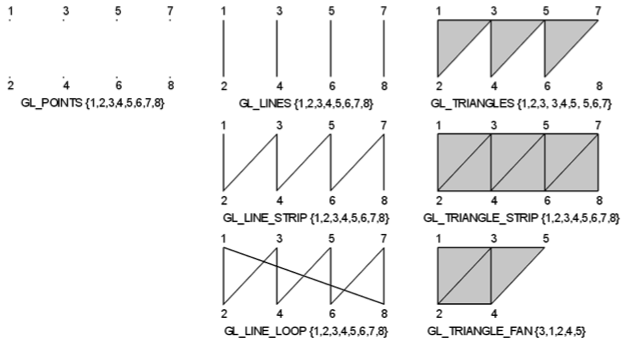
\includegraphics[scale=0.4]{opengl_primitive.png}
\end{center}
\subsection{DrawElements}
Mit dem Zeichnungsbefehl \textbf{glDrawArrays} werden OpenGL-Primitive direkt mit der Vertex-reihenfolge erzeugt. Wird ein Vertex mehrfach in der Geometrie verwendet, so muss er also auch mehrfach im Array vorhanden sein. \\
\\
Mit dem Zeichnungsbefehl \textbf{glDrawElements} werden OpenGL-Primitive anhand eines Index-Arrays gezeichnet. Ein mehrfach vorkommender Vertex muss so nur einmal im Array vorkommen und kann via Index mehrfach referenziert werden. Die Vertexposition verbraucht immerhin 12 Bytes, während ein Index je nach unsigned Datentyp nur 1-4 Bytes belegt.
\lstinputlisting[style=CStyle,caption=Draw Elements]{drawElements.c}

\subsection{Vertex Buffer Object}
Mit jedem Aufruf der Zeichnungsbefehle \textbf{glDrawArrays} und \textbf{glDrawElements} werden die Vertex-Arrays vom Hauptspeicher über den Datenbus auf die Grafikkarte kopiert. Dies ist unumgänglich, wenn sich die Vertexdaten sehr schnell ängern würden. Die allermeisten Objekte bleiben aber über viele Frames, wenn nicht gar für immer gleich. Auch wenn die Objekte sich bewegen, so ändern wir ja nur Transformationsmatrizen und nicht die Struktur der Dreiecksnetze. Es wprde also Sinn machen, wenn wir die Vertex-Arrays im RAM der Grafikkarte speichern könnten und der Kopiervorgang nur einmal durchgeführt werden müsste. Genau diese Möglichkeit bieten uns die Vertex Buffer Objekte.
\lstinputlisting[style=CStyle,caption=VBO erstellen]{buildVBO.c}

\newpage
\section{Shader}
\subsection{Shader Programme kompilieren, linken \& aktivieren}
\begin{center}
	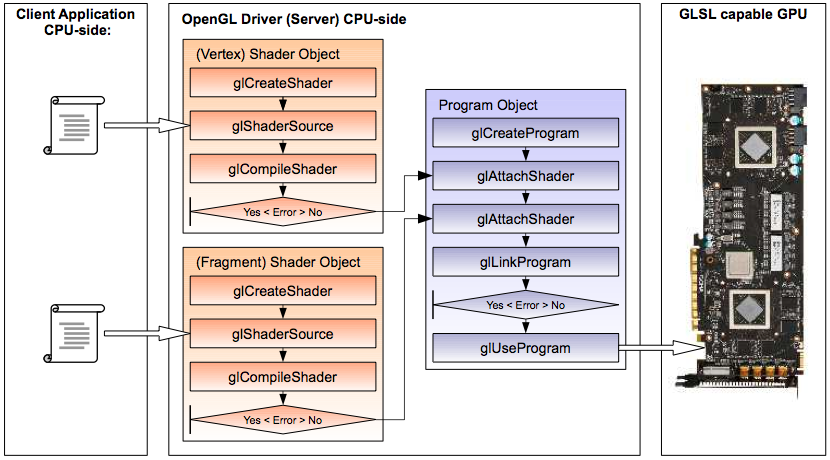
\includegraphics[scale=0.5]{shader.png}
\end{center}
\subsection{einfache Datentypen}
\lstinputlisting[style=CStyle,caption=Datentypen]{glsl_simpleDatatype.c}
\subsection{Typen Qualifizierer}
\subsubsection{const}
\begin{itemize}
	\item Konstanten müssen bei der Deklaration initialisiert werden.
	\item Kann benutzerdefiniert sein.
	\item Kann vordefiniert sein durch GLSL.
\end{itemize}
\subsubsection{attribute}
Mit attribute qualifizierte Variablen dienen als Übergabeparameter der Vertex-Attribute vom Hauptprogramm ans Vertex-Programm. Die Werte können mit jedem Vertex ändern.
\subsubsection{uniform}
Als uniform qualifizierte Variablen dienen als Übergabeparameter vom Hauptprogramm in ein Vertex- oder Fragment-Programm. Deren Werte bleiben für einen ganzen Zeichnungsbefehl konstant.
\subsubsection{varying}
Als varying qualifizierte Variablen dienen als Übergabeparameter vom Vertex- zum Fragment-Programm. Der Wert einer Varying-Variable wird im Vertex-Programm gesetzt und steht dann über das Primitiv interpoliert im Fragment-Programm zur Verfügung.
\begin{center}
	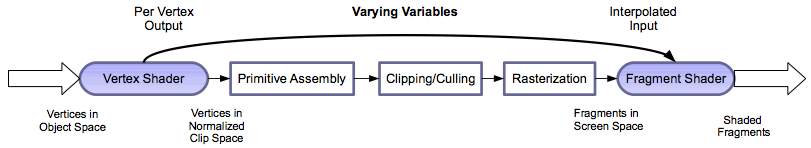
\includegraphics[scale=0.5]{glsl_varying.png}
\end{center}

\newpage
\section{Beleuchtung}
\subsection{Lichtquellen}
\begin{center}
	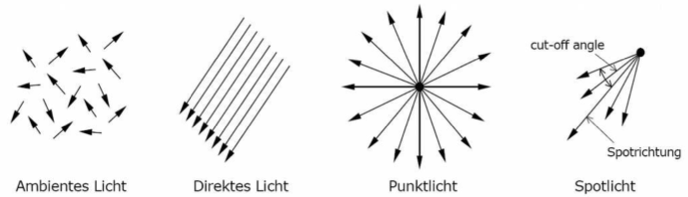
\includegraphics[scale=0.5]{lichtquellen.png}
\end{center}
\subsection{Reflexion}
\subsubsection{Ambiente Reflexion}
$I_a$ bezeichnet darin die konstante, ambiente Lichtintensität und $k_a$ den ambienten Reflexionskoeffizienten (zw. 0 und 1) des reflektierenden Materials. 
\begin{equation}
I_{ambi}=I_a * k_a
\end{equation}
\subsubsection{Diffuse Reflexion}
$I_d$ bezeichnet darin die konstante, diffuse Lichtintensität und $k_d$ den diffusen Reflexionskoeffizienten (zw. 0 und 1). Wenn N und L normalisiert sind, kann der Kosinus durch das Skalarprodukt beider Vektoren ersetzt werden.
\begin{equation}
I_{diff}=I_d * k_d * max( cos(\theta), 0) = I_d * k_d * max(N \bullet L, 0)
\end{equation}
\begin{center}
	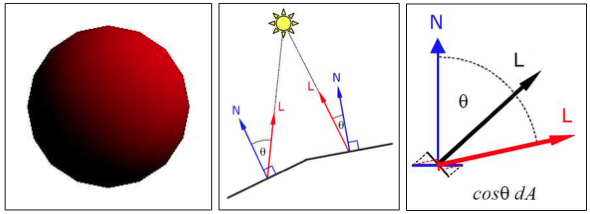
\includegraphics[scale=0.4]{diffuse_reflexion.png}
\end{center}
\subsubsection{Spiegelnde Reflexion}
Die Menge des reflektierten Lichts ist vom Beobachterstandpunkt abhängig bzw. vom Winkel $\alpha$ zwischen dem Beobachtungsvektor E (eye) und dem reflektierten Strahl R, sowie von einer Materialbeschaffenheit $n$ bezüglich der Reflektierbarkeit (Shininess) ab. $I_s$ bezeichnet die konstante, spiegelnde Lichtintensität und $k_s$ den spiegelnden Reflexionskoeffizienten (zw. 0 und 1).
\begin{equation}
I_{spec}=I_s * k_s * max( cos(\alpha), 0)^n = I_s * k_s * max(R \bullet E, 0)^n
\end{equation}
\begin{center}
	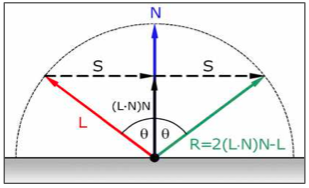
\includegraphics[scale=0.4]{reflektierender_strahl.png}
	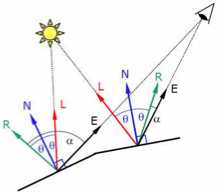
\includegraphics[scale=0.4]{spiegelnde_reflexion.png}
\end{center}
\subsubsection{Lichtabnahme (Attenuierung)}
Bevor wir alles zusammenstellen können, müssen wir noch die Energieabnahme des Lichts (Lichtabnahme) in Abhängigkeit der Distanz berücksichtigen. Darin sind $c_1$, $c_2$ und $c_3$ Konstanten für die konstante, die lineare und die quadratische Lichtabnahme in Abhängigkeit der Distanz $d$. Diese Lichtabnahme wirkt nur auf die diffuse und die spiegelnde Reflexion.
\begin{equation}
f_{att}=min(\frac{1}{c_1 + c_2 * d + c_3 * d^2}, 1)
\end{equation}
\subsection{Beleuchtungsmodell nach Phong}
\begin{equation}
	I_{Phong}=I_{amb} + \sum_{i=0}^{lights-1} f_{att} * (I_{diff} + I_{spec})
\end{equation}
\subsection{Erweiterungen im alten OpenGL Beleuchtungsmodell}
\begin{equation}
	I_{OpenGL}=k_e + I_{aglobal} * k_{aglobal} + \sum_{i=0}^{lights-1} f_{att} *  S_{spott} * (I_{ambi} + I_{diff} + I_{spec})
\end{equation}
\begin{description}
	\item[Emittierende Farbintensität] $k_e$ für selbststrahlende Objekte
	\item[Globale ambiente Hintergrundintensität] $I_{aglobal}$ unabhängig von einer Lichtquelle
	\item[Spotlichteffekt] $S_{spot}$ bewirkt die Begrenzung des Spotlichts und eine Lichtabnahme innerhalb des Lichtkegels von der Spotachse zum Kegelrand bewirkt. Der Wert von Sspoteffect ist:
	\begin{itemize}
		\item 1, wenn das Licht kein Spotlicht ist (Cut-Off Winkel=180).
		\item 0, wenn das Licht ein Spotlicht ist, der Vertex aber ausserhalb des Spotkegels ist.		
		\item $max(L \bullet S , 0)^{spotexp}$ , wobei L der Vektor von der Vertexposition zum Licht ist und S die Spotrichtung und spotexp ein Exponent zwischen 0 und 128. Standardwert ist 0.
		\item Ein zunehmender Exponent bewirkt eine Abnahme des Lichtes zum Kegelrand.
	\end{itemize}
\end{description}
\subsection{Blinn's Halbvektor}
Jim Blinn steuerte eine vereinfachte Berechnung des spekulären Anteils bei, indem er den Winkel zwischen der Normalen N und einem Halbvektor H berechnet. H ist der normalisierte Halbvektor zwischen der Blickrichtung E und der Lichtrichtung L.
\begin{equation}
I_{specBlinn}=I_s * k_s * max(N \bullet H ,0)^n
\end{equation}
\begin{equation}
(R \bullet E)^n \approx (N \bullet H)^{4n}
\end{equation}
\subsection{Schattierung}
\subsubsection{Berechnung pro Dreieck: Flat Shading}
Im alten OpenGL war es möglich die Beleuchtungsrechnung auf den letzten Vertex eines Polygons zu beschränken. Dies bewirkte eine flache Schattierung und war die einfachste und schnellste Beleuchtung.
\subsubsection{Berechnung pro Vertex: Gouraud Shading}
Im alten OpenGL wurde die Blinn'sche Version des Phong Modells pro Vertex gerechnet und die Farbwerte dann über das Polygon interpoliert. Dabei werden die Farbwerte zwischen den Eckpunkten eines Polygons linear interpoliert. Der Scanline Algorithmus wird ist in folgende Schritte gegliedert:
\begin{enumerate}
	\item An allen Ecken eines Dreiecks müssen die Normalen definiert sein, die aus den Flächennormalen der jeweiligen Nachbardreiecke gemittelt wurden.
	\item Die Farbwerte an den Ecken gemäss Beleuchtungsmodell bestimmen.
	\item Pixelzeile für Pixelzeile werden die Kantenwerte linear interpoliert.
	\item Pixelintensitäten berechnen durch Interpolation zwischen den Werten.
\end{enumerate}
\textbf{Nachteile}:
\begin{itemize}
	\item  Ungenaue Glanzlichter
	\item Keine Lichtkegel
	\item Keine perspektivische Verzerrungen
	\item Abhängigkeit von der Orientierung
	\item Nicht repräsentative Knotennormalen
\end{itemize}
\begin{center}
	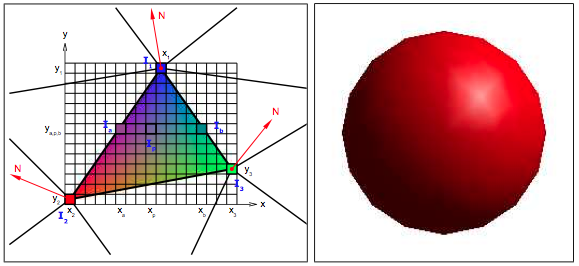
\includegraphics[scale=0.4]{gouraud_shading.png}
\end{center}
\subsubsection{Berechnung pro Pixel: Phong Shading}
Es liegt auf der Hand, dass die Phong Shading wesentlich aufwendiger ist, wenn die gesamte Rechnung pro Pixel anstatt nur pro Vertex gemacht werde muss. Zusätzlich muss ja vorgängig für jedes Pixel eine interpolierte Normale und Pixelposition berechnet werden. \\
\\
\textbf{Nachteile}:
\begin{itemize}
	\item Polygonale Silhouetten
	\item Spotlichtgrenzen nicht auf Kugeloberflächen
\end{itemize}
\begin{center}
	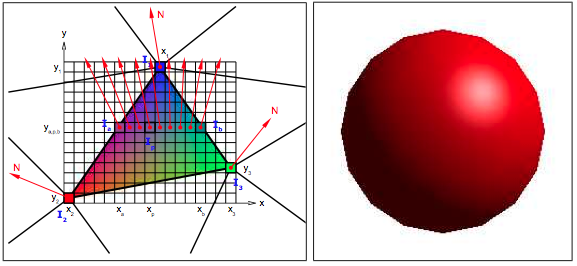
\includegraphics[scale=0.4]{phong_shading.png}
\end{center}

\newpage
\section{Texture Mapping}
\subsection{verschiedene Texturen}
\begin{center}
	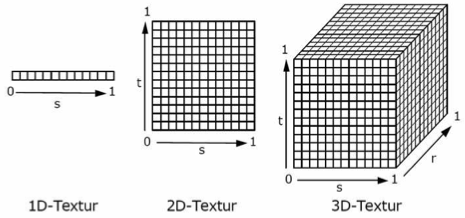
\includegraphics[scale=0.4]{texturen.png}
\end{center}
\subsection{Textur Abbildung}
\begin{center}
	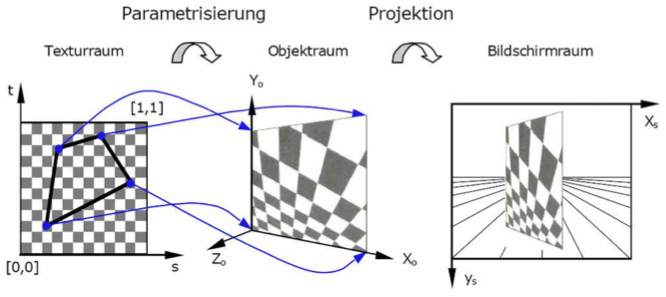
\includegraphics[scale=0.4]{textur_abbildung.png}
\end{center}
\subsection{Texturfilterung}
\begin{center}
	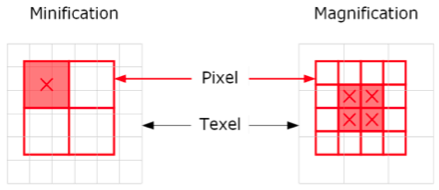
\includegraphics[scale=0.4]{texture_sampling.png}
\end{center}
\subsubsection{Point Sampling}
Wird keine Filterung angewendet, so wird nach der Point Sampling oder Nearest Neighbour Methode gearbeitet, bei der das dem Pixelzentrum (Kreuz) am nächsten liegende Texel verwendet wird. Dies ist also im Prinzip nur ein Abschneiden der Nachkommastellen.
\subsubsection{Bilineare Filterung}
Bei der bilinearen Filterung werden die benachbarten Texel mit berücksichtigt. Da in X- und Y-Richtungen interpoliert wird, nennt man diesen Filter bi-linear.
\begin{center}
	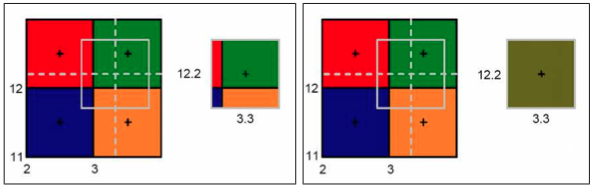
\includegraphics[scale=0.4]{bilineare_filterung.png}
\end{center}
\subsubsection{MIP-Mapping}
Die Idee dahinter ist, eine Textur bereits vor der Anwendung mit mehreren Verkleinerungen anzulegen, um diese je nach Distanz zum Betrachter einzusetzen.
\begin{center}
	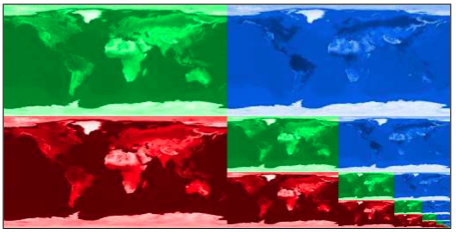
\includegraphics[scale=0.4]{mip-mapping.png}
\end{center}
\subsubsection{Trilineare Filterung}
Der Übergang von einem MIP-Level zum nächsten fällt besonders bei grossen Flächen mit gleicher Textur auf. Die verschieden aufgelösten MIP-Level bilden dabei eine scharfe Kante. Beim trilinearen Filtern werden nun zuerst die entsprechenden Texel der zwei MIP- Levels bilinear gefiltert und diese dann noch einmal linear (eben tri) zwischen den beiden MIP-Levels.
\begin{center}
	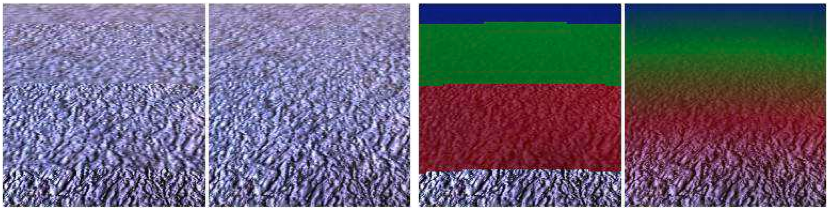
\includegraphics[scale=0.4]{trilineare_filtering.png}
\end{center}
\subsubsection{Anisotropische Filterung}
Die trilineare Filterung hat nur noch einen Mangel. Die perspektivische Verzerrung wird zwar bei der Bestimmung der Texel-Position berücksichtigt, bei der bilinearen Interpolation fällt sie aber unter den Tisch. Man müsste Texturen, auf die man sehr schräg sieht, mit anderen Verfahren filtern als jene, auf die man senkrecht sieht. Da für beste Qualität nicht mehr isotrop, also gleichmässig gefiltert werden kann, muss das ungleichmässig (sprich anisotrop) getan werden. Beim bilinearen Filtern werden bekanntlich nur 4 Texel gemischt. Für den trilinearen Filter sind 2 bilinear gefilterte Texel.
\begin{center}
	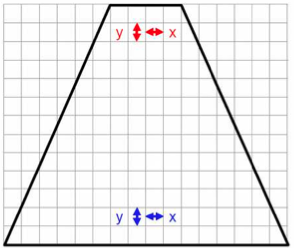
\includegraphics[scale=0.4]{anisotropische_filterung.png}
\end{center}

\subsection{Bump Mapping}
\begin{center}
	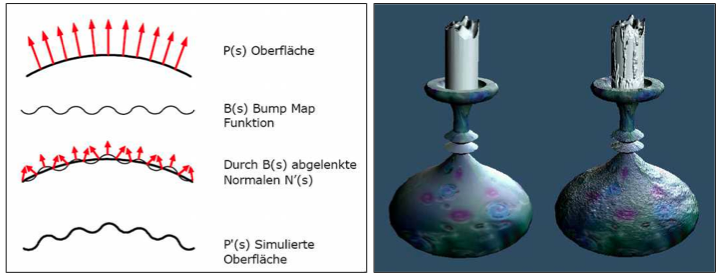
\includegraphics[scale=0.3]{bump_mapping.png}
\end{center}
\subsubsection{Heightfield Bump Mapping}
Die Normale wird durch einen Vektor D abgelenkt, indem er zur Normalen hinzuaddiert wird. Der Ablenkungsvektor D berechnet sich aus den Tangentialvektoren T und B (Binormale) sowie aus der partiellen Ableitung d (= Grauwertsteigung) bei der Texturkoordinate s,t in der Bumpmap.
\begin{center}
	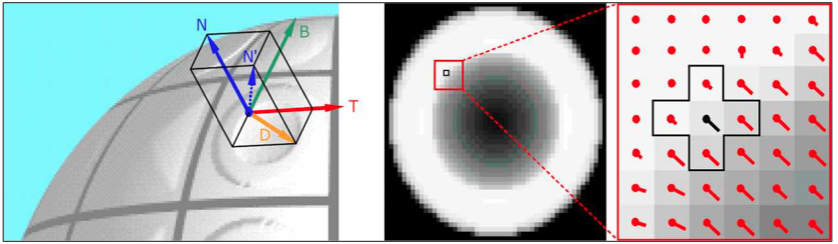
\includegraphics[scale=0.4]{heightfield_bump_mapping.png}
\end{center}
\subsubsection{Normalmap Bump Mapping}
Eine Verbesserung hinsichtlich der Performanz ist das sogenannte Normalmap Bump Mapping. Dabei wird die bereits abgelenkte Normale im Tangentenraum in einem RGB- Bild abgespeichert. Die Koordinatenkomponenten x, y und z entsprechen den Farbkomponenten r, g und b.
\begin{center}
	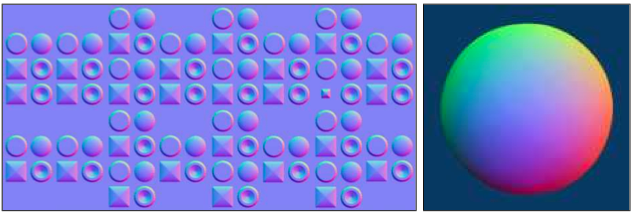
\includegraphics[scale=0.4]{normalmap_bump_mapping.png}
\end{center}
\subsubsection{Parallax Mapping}
Die Grundidee besteht darin die Texturkoordinaten (im Bild neben an nur die T-Komponente) so zu dehnen, dass wir sie den Höhen entsprechend richtig sehen. Für den Punkt P im Bild neben an würden wir ohne Parallax Mapping das Texel bei T erhalten, obwohl wir eigentlich die Farbe bei $T_I$(deal) sehen sollten. Um diese Berechnung zu vereinfachen, beschränkt man den Versatz um die Höhe H entlang des Augvektors E.
\begin{center}
	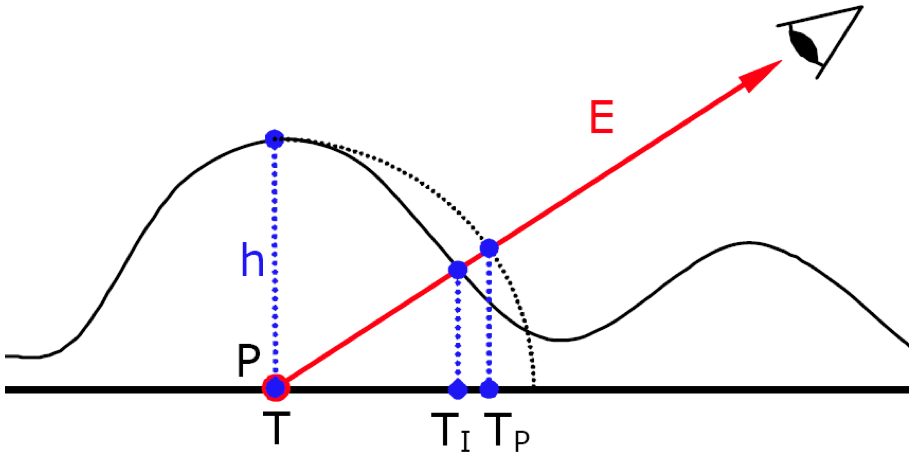
\includegraphics[scale=0.2]{parallax_mapping.png}
\end{center}

\subsection{Texture Mapping in OpenGL}
\begin{enumerate}
	\item Texturnamenanlegen.
	\item Textur binden(aktivieren). 
	\item Texturparameter setzen. 
	\item Texturdaten übergeben
	\item Mipmap-Level generieren.
\end{enumerate}

\newpage
\section{Frustum Culling}
\subsection{Ziel}
Ziel ist es, nur Objekte durch die Pipeline zu schicken, die sichtbar sind:
\begin{center}
	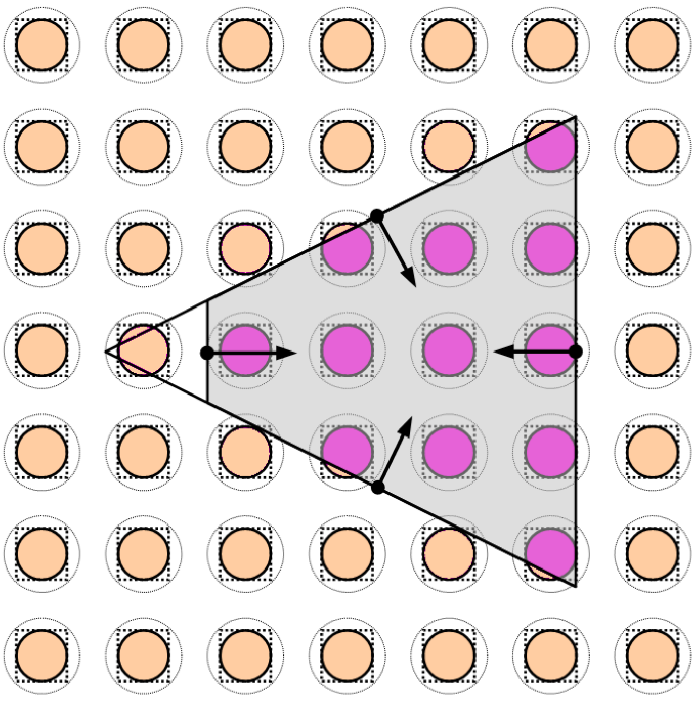
\includegraphics[scale=0.2]{frustum_culling.png}
\end{center}
\subsection{Hüllvolumen}
Die Wahl des Hüllvolumens hängt von folgenden Kriterien ab:
\begin{itemize}
	\item Passgenauigkeit des Hüllvolumens
	\item Kosten des Hüllvolumenschnitttests. 
	\item Erstellungskosten des Hüllvolumens.
\end{itemize}
\begin{center}
	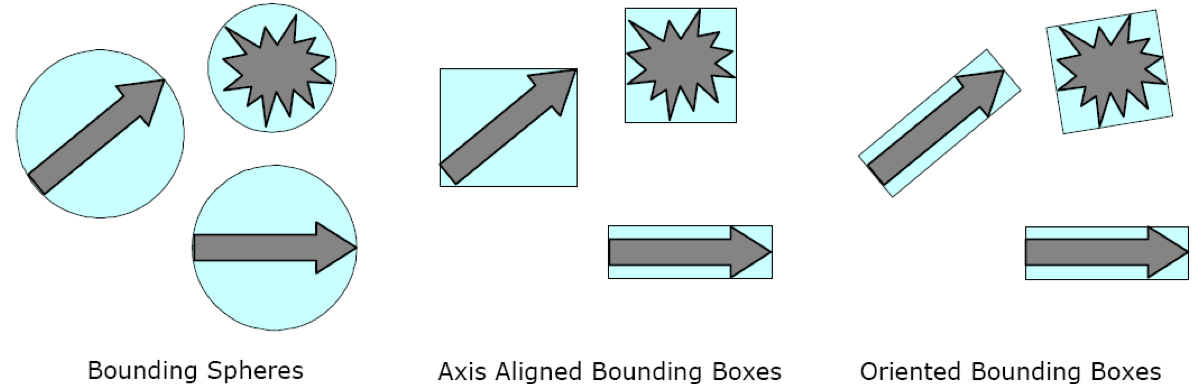
\includegraphics[scale=0.3]{huellvolumen.png}
\end{center}

\newpage
\section{Alpha Blending}
\subsection{Einleitung}
\begin{itemize}
	\item Beim Alpha Blending wird eine neue Frabe mit der bestehenden vermischt.
	\item Der Alpha Wert ist der Dekungsgrad.
	\item Der Alpha Wert der Farbe ist der 4. Parameter bei den Farbangaben RGBA.
\end{itemize}
\subsection{Blendfunktion}
\begin{itemize}
	\item Die Blendfunktion bestimmt, wie die bestehende Farbe ($R_D$ $G_D$ $B_D$ $A_D$) mit der Neuen ($R_S$ $G_S$  $B_S$ $A_S$) kombiniert wird.
	\item Der resultierende Farbe entsteht durch komponentenweise Addition, wobei man jede Komponente über die Source- bzw. Destination-Faktoren beeinflussen kann: \\
	$RGBA = ((R_SS_R + R_DD_R), (G_SS_G + G_DD_G), (B_SS_B + B_DD_B), (A_SS_A + A_DD_A))$
\end{itemize}
\subsection{Additive Blending}
\begin{center}
	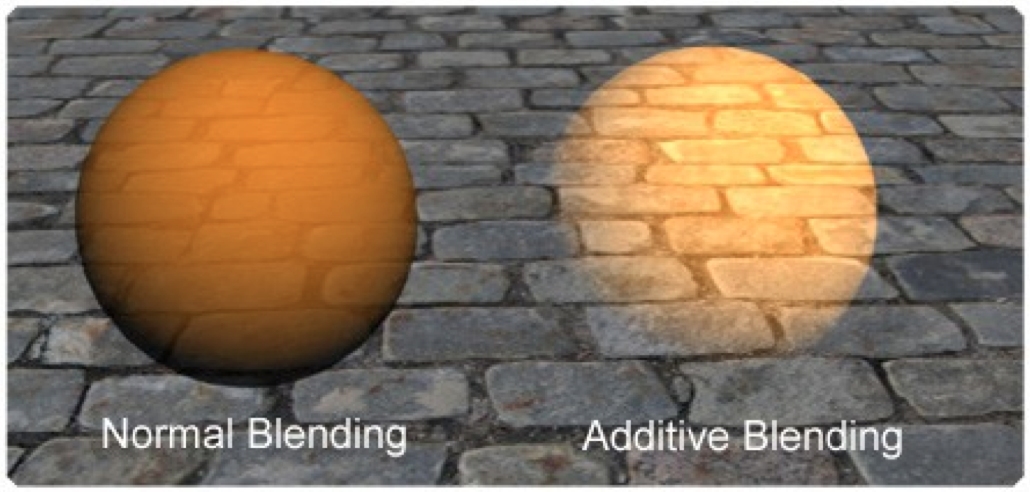
\includegraphics[scale=0.2]{additive_blending.png}
\end{center}
\subsection{Zeichnungsreihenfolge}
Zeichnungsreihenfolge ist entscheidend:
\begin{enumerate}
	\item Alle opaqen (=nicht-transparente) Objekte
	\item Alle transparenten Objekte
\end{enumerate}
\begin{center}
	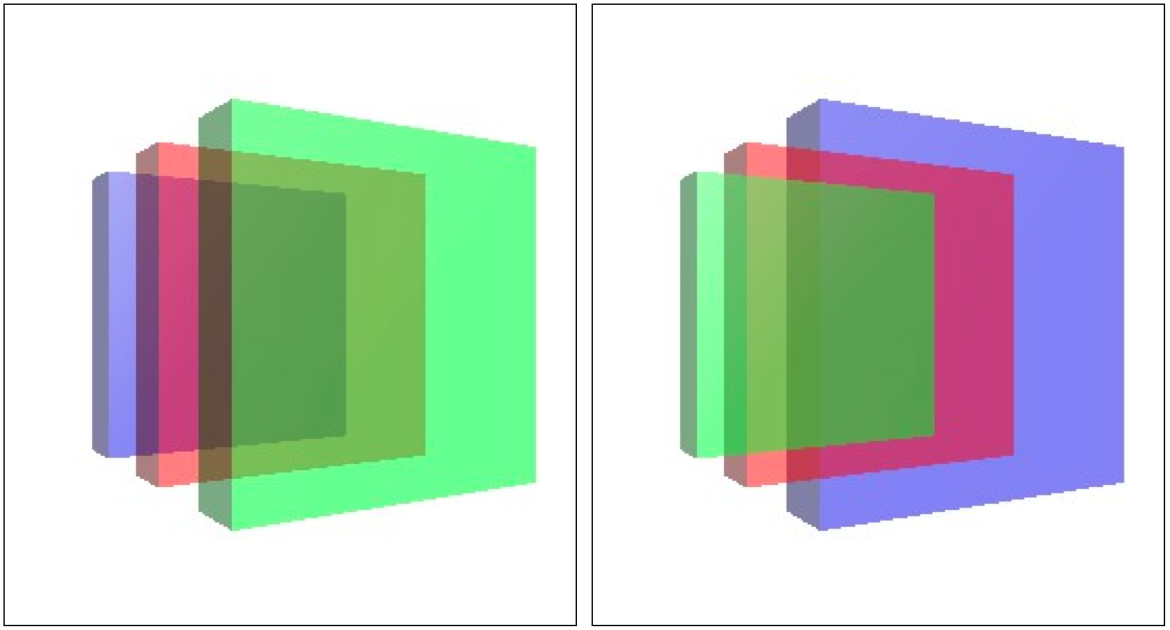
\includegraphics[scale=0.2]{alphablending_order.png}
\end{center}

\newpage
\section{Deferred Shading}
Methode um in dreidimensionalen Szenen die Geometrieverarbeitung von der Lichtberechnung zu trennen. So sind mehrere hundert dynamische Lichter in geometrisch komplexen Szenen möglich
\subsection{Prinzip}
In klassischen Rendermethoden wird anhand von Tiefe (depth), Ausrichtung (normals) und Farbe (albedo) eines Eckpunktes und Farbe, Intensität und Einfallswinkel einer Lichtquelle der finale Farbwert für den jeweiligen Eckpunkt ermittelt. Für jede Lichtquelle muss so jeder Eckpunkt zur Berechnung herangezogen werden. \\
Beim Deferred Shading werden nun Tiefenwert, Ausrichtung und Farbe eines jeden Pixels in jeweils eine Textur in Bildschirmgröße gespeichert. Dies wird durch sogenannte Multiple Render Targets ermöglicht, wobei in jedem Rendervorgang in verschiedene Framebufferobjekte (die Texturen) gleichzeitig geschrieben werden kann. Statt dass nun jeder Eckpunkt mit den Lichtquellen verrechnet werden muss, muss nur noch jedes Pixel (in dem alle benötigten Werte – depth, normals und albedo – vorhanden sind) bei der Berechnung berücksichtigt werden. \\
Die Berechnung selbst erfolgt durch klassische Beleuchtungsmodelle, wie zum Beispiel nach Phong. Dabei kann zusätzlich noch Glanzlicht mit einbezogen werden. Technisch geschieht das im Pixel- bzw. Fragment-Shader am Ende der Grafikpipeline.
\subsection{Vorteile}
\begin{itemize}
	\item Independent of scene complexity \& dynamics.
	\item Fully in hardware.
	\item Well suited for deferred renderers (as normal map is typically available).
\end{itemize}
\subsection{Nachteile}
\begin{itemize}
	\item Noise removal requires extra blur stage.
	\item Limited range of sample sphere makes approach relatively local and view dependent.
\end{itemize}
\subsection{OpenGL}
\subsubsection{Framebuffer objects}
\begin{itemize}
	\item FBOs encapsulate a framebuffer that can be used for off- screen rendering.
	\item Each FBO has a given dimension, and a number of attachments (n color buffers, depth buffer, and stencil buffer).
	\item Attached buffers are either textures or renderbuffers. 
	\item FBOs can be enabled for writing and reading.
\end{itemize}
\subsubsection{FBO relevant API}
\begin{itemize}
	\item glGenFramebuffer, glDeleteFramebuffers
	\item glBindFramebuffer - Bind for reading or writing
	\item glClearBuffer
	\item glFramebufferTexture2D - Attach texture to FBO
	\item glCheckFramebufferStatus -  Important: Check if FBO is correctly set up
\end{itemize}

\newpage
\section{Shadow Rendering}
\subsection{Einleitung}
\begin{itemize}
	\item Schatten für Echtzeitanwendungen werden normalerweise mit Deferred Rendering implementiert
	\item In einem ersten Schritt werden Informationen gesammelt die dann für die Beleuchtungsberechnung in einem zweiten Schritt verwendet werden
\end{itemize}
\subsection{Shadow Volumes}
\begin{itemize}
	\item Jedes Polygon erzeugt ein Schattenvolumen (Pyramidenstumpf)
	\item Für jeden Sichtstrahl wird ein Zähler inkrementiert beim Eintreten in das Schattenvolumen und dekrementiert beim Austreten.
	\item Zonen mit einem Zähler == 0 sind beleuchtet, != 0 sind im Schatten
	\item Wie kann man das erreichen ohne Ray-Tracing?
\end{itemize}
\subsection{Shadow Maps}
\begin{itemize}
	\item Rendern der Szene um Farb- und Tiefenwerte zu erhalten
	\item Rendern der Shadow Volumes
	\item Kombinieren der Resultate
\end{itemize}
\subsection{Variance Shadow Maps}
\begin{itemize}
	\item Multisampling vermeiden, Filter der GPU verwenden
	\item Wie bei PCF interessiert uns der Zusammenhang der Shadow Map Werte einer Region und des Tiefenwerte des Fragments das wir zeichnen
	\item Statt Shadow Map Anteile (PCF) betrachtet man die Verteilung der Tiefenwerte
	\item Die Tschebyscheff-Ungleichung liefert uns die Wahrscheinlichkeit bei bekanntem Mittelwert und Varianz ob ein Wert  auftritt oder nicht
\end{itemize}
\subsection{Cascade Shadow Maps}
\begin{center}
	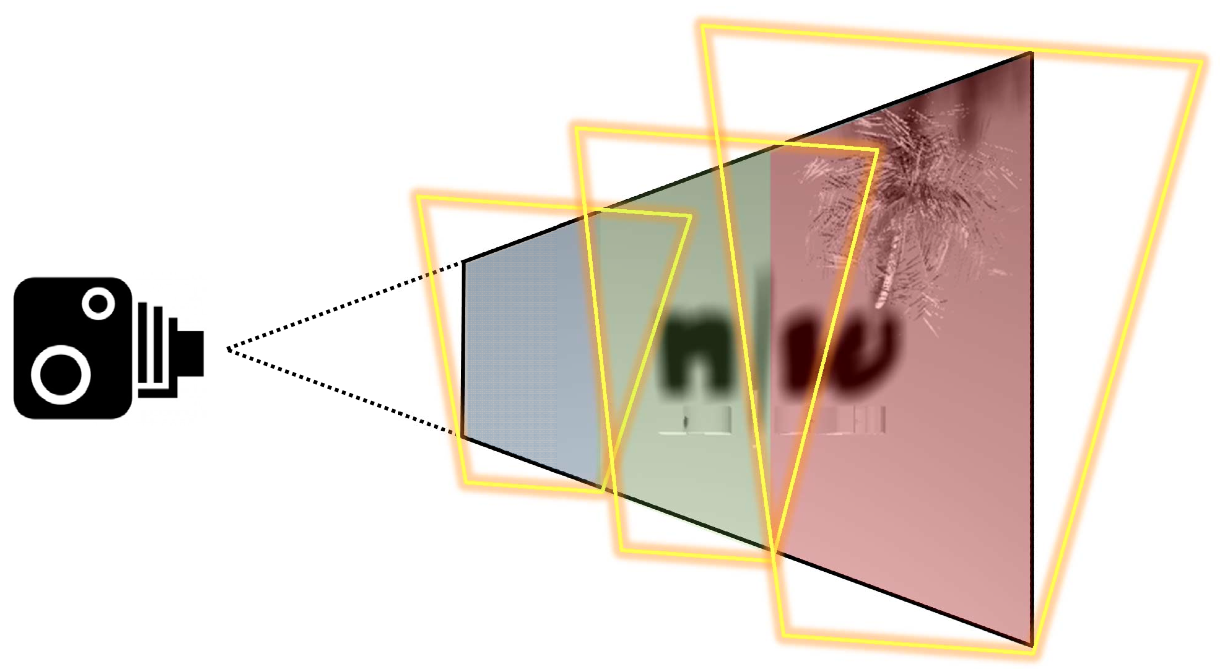
\includegraphics[scale=0.2]{cascade_shadow_maps.png}
\end{center}
\subsection{Vergleich}
\begin{center}
	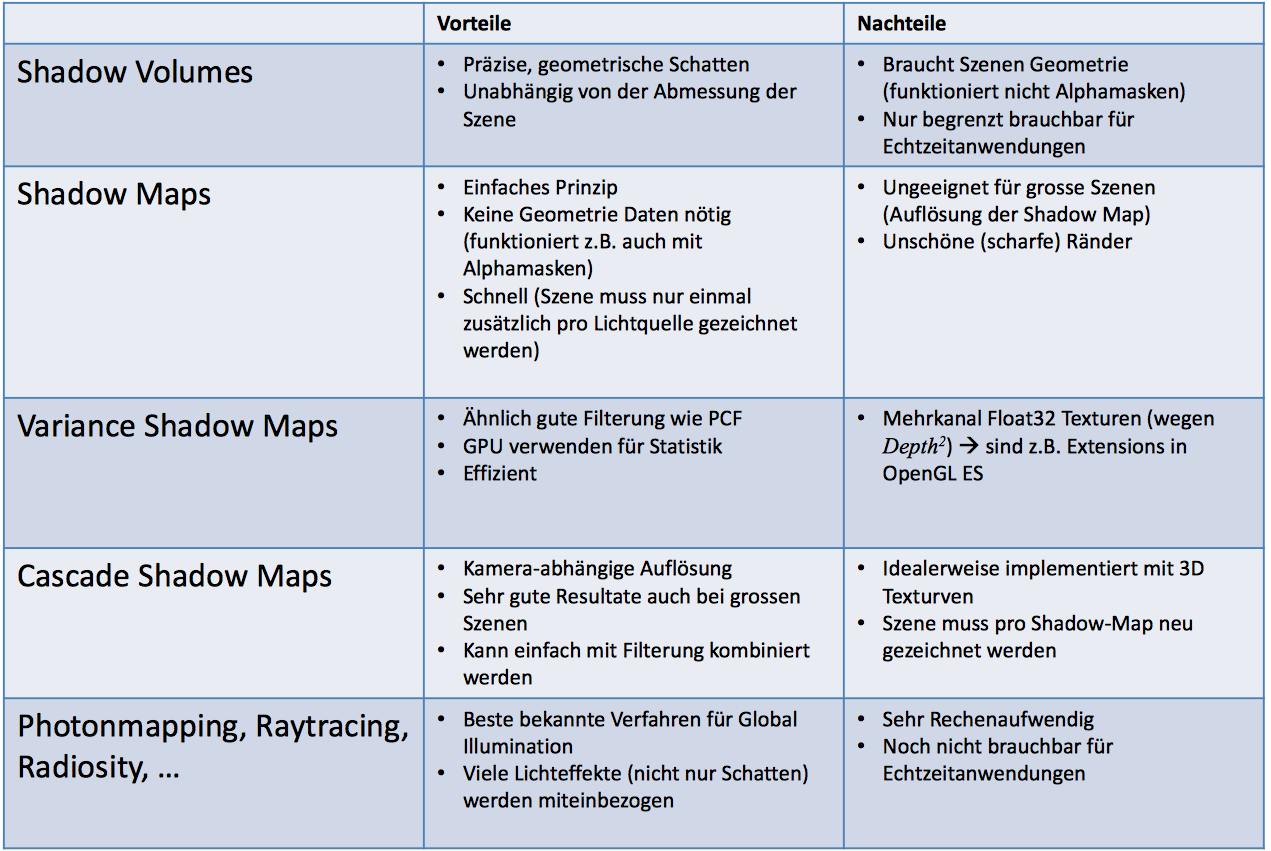
\includegraphics[scale=0.4]{shadow_rendering.png}
\end{center}
% Inhalt Ende 
\end{document} 